% Options for packages loaded elsewhere
\PassOptionsToPackage{unicode}{hyperref}
\PassOptionsToPackage{hyphens}{url}
\PassOptionsToPackage{dvipsnames,svgnames,x11names}{xcolor}
\documentclass[
]{ltjsarticle}
\usepackage{xcolor}
\usepackage[margin=20mm]{geometry}
\usepackage{amsmath,amssymb}
\setcounter{secnumdepth}{-\maxdimen} % remove section numbering
\usepackage{iftex}
\ifPDFTeX
  \usepackage[T1]{fontenc}
  \usepackage[utf8]{inputenc}
  \usepackage{textcomp} % provide euro and other symbols
\else % if luatex or xetex
  \usepackage{unicode-math} % this also loads fontspec
  \defaultfontfeatures{Scale=MatchLowercase}
  \defaultfontfeatures[\rmfamily]{Ligatures=TeX,Scale=1}
\fi
\usepackage{lmodern}
\ifPDFTeX\else
  % xetex/luatex font selection
\fi
% Use upquote if available, for straight quotes in verbatim environments
\IfFileExists{upquote.sty}{\usepackage{upquote}}{}
\IfFileExists{microtype.sty}{% use microtype if available
  \usepackage[]{microtype}
  \UseMicrotypeSet[protrusion]{basicmath} % disable protrusion for tt fonts
}{}
\makeatletter
\@ifundefined{KOMAClassName}{% if non-KOMA class
  \IfFileExists{parskip.sty}{%
    \usepackage{parskip}
  }{% else
    \setlength{\parindent}{0pt}
    \setlength{\parskip}{6pt plus 2pt minus 1pt}}
}{% if KOMA class
  \KOMAoptions{parskip=half}}
\makeatother
\usepackage{longtable,booktabs,array}
\newcounter{none} % for unnumbered tables
\usepackage{calc} % for calculating minipage widths
% Correct order of tables after \paragraph or \subparagraph
\usepackage{etoolbox}
\makeatletter
\patchcmd\longtable{\par}{\if@noskipsec\mbox{}\fi\par}{}{}
\makeatother
% Allow footnotes in longtable head/foot
\IfFileExists{footnotehyper.sty}{\usepackage{footnotehyper}}{\usepackage{footnote}}
\makesavenoteenv{longtable}
\usepackage{graphicx}
\makeatletter
\newsavebox\pandoc@box
\newcommand*\pandocbounded[1]{% scales image to fit in text height/width
  \sbox\pandoc@box{#1}%
  \Gscale@div\@tempa{\textheight}{\dimexpr\ht\pandoc@box+\dp\pandoc@box\relax}%
  \Gscale@div\@tempb{\linewidth}{\wd\pandoc@box}%
  \ifdim\@tempb\p@<\@tempa\p@\let\@tempa\@tempb\fi% select the smaller of both
  \ifdim\@tempa\p@<\p@\scalebox{\@tempa}{\usebox\pandoc@box}%
  \else\usebox{\pandoc@box}%
  \fi%
}
% Set default figure placement to htbp
\def\fps@figure{htbp}
\makeatother
\setlength{\emergencystretch}{3em} % prevent overfull lines
\providecommand{\tightlist}{%
  \setlength{\itemsep}{0pt}\setlength{\parskip}{0pt}}
\usepackage{float}
\floatplacement{figure}{H}
\usepackage{bookmark}
\IfFileExists{xurl.sty}{\usepackage{xurl}}{} % add URL line breaks if available
\urlstyle{same}
\hypersetup{
  colorlinks=true,
  linkcolor={Maroon},
  filecolor={Maroon},
  citecolor={Blue},
  urlcolor={Blue},
  pdfcreator={LaTeX via pandoc}}

\author{}
\date{}

\begin{document}

\section{Paper 0: Distortion of the Geodesic Unit Cell in
Positively-Curved Constant-Curvature Space --- Exact Evaluation of Edge,
Angle, Area, and
Volume}\label{paper-0-distortion-of-the-geodesic-unit-cell-in-positively-curved-constant-curvature-space-exact-evaluation-of-edge-angle-area-and-volume}

\textbf{Author}: Noriaki Kihara \textbf{Affiliation}: WF System Co.,
Ltd.~/ ORCID: 0009-0004-6753-4020 \textbf{DOI}: Version
10.5281/zenodo.20684135 (this version) / Concept 10.5281/zenodo.20680269
(cite this; always resolves to the latest version) \textbf{Zenodo}:
https://zenodo.org/records/20684135 \textbf{Version}: v1.4 (v1.3 plus a
prior-work paragraph in §4.6 {[}differentiation from spectral dimension,
Böröczky, Schläfli{]} with external references, a one-sentence Schläfli
positioning of the existence threshold in §1, and a fix of the Appendix
A math typesetting to proper LaTeX. v1.3 inserted five exact-computation
figures into v1.2. All figures are exact computations, no schematics.
Two-party verification protocol.) \textbf{Position}: This is the
Foundations volume, \textbf{Paper 0}; its correction target is the flat
counting of Papers 1--2 (§5). Adding the Paper 0 row to 論文一覧.md /
the survey references, and the cross-link with Paper 1, are handled
separately as publication management (after this paper is finalized).
\textbf{Seven viewpoints}: edge (1), vertex angle (2), area (3), volume
(4), inverse curvature (4.5), dimensional ambiguity and conjugate
quantity (4.6), dimensional emergence and the d=4 lock (4.7). All
numbers are reproducible with the bundled script; all 6 verification
items pass. \textbf{Series}: The dual geometry of wavelength space and
frequency space (Foundations volume, Paper 0) \textbf{Verification
script}: \texttt{paper0\_geodesic\_cell\_distortion.py}

\begin{center}\rule{0.5\linewidth}{0.5pt}\end{center}

\subsection{0. Position of this paper --- a precise definition of the
distortion
problem}\label{position-of-this-paper-a-precise-definition-of-the-distortion-problem}

Up to now this series has used, as its base map, the spherical
projection σ\_R(x)=(R/‖x‖)x (Spherical-projection note
``Central-projection series: the base map radial projection σ\_R,''
Concept DOI 10.5281/zenodo.20462569 --- an external reference in a
series separate from this one (Papers 1--16); treated as out-of-series
literature not listed in 論文一覧.md), together with the central
projection Φ\_R, its restriction to the tangent hyperplane Π\_R
(Central-projection note). σ\_R preserves direction and angle but not
distance, and its distortion ``does not appear at a single point; it
becomes manifest only as a relation between points (relative
configuration, spacing)'' (Spherical-projection note, Observation 2.7).
\textbf{However, writing this distortion down quantitatively as edge,
vertex angle, area, and volume has never been clearly formalized in any
paper} --- §4.3 of the Spherical-projection note explicitly deferred the
formulation in terms of induced metric and curvature to a separate
paper, and the counting from Paper 1 onward proceeded with the flat
norm, without incorporating the intrinsic curvature of the surface
S\^{}d(R) defined by the constraint Σν\(^{2}\)=\(\mathcal{N}\)\(^{2}\)
into the 4-degree-of-freedom count.

\textbf{The aim of this paper is to define this deferred ``distortion
problem'' --- the geometric distortion of a unit cell placed in a
positively-curved constant-curvature space of curvature radius R ---
clearly, as an elementary calculation in differential geometry.} But an
important refinement comes first: the flat treatment of Papers 1--2 is
\textbf{not a deficiency; for 1-dimensional-wave content it is
curvature-exact} (§2: d=1 is intrinsically flat with zero distortion;
§4.8). Distortion (§3--4, d≥2) appears only in true geodesic cells that
couple several axes, and that is precisely the regime the series handles
with amplitude-free logic waves (Paper 9 §2.3 ``curvature
consistency''). The correct reading of this paper is ``demarcation of
the boundary within which the flat treatment is exactly valid''; the
correction in §5 is limited to a mean-field estimate for the
reinterpretation into multi-dimensional geodesic cells. No probability,
measure, or amplitude appears. The single question is:

\begin{quote}
Under canonicalization (discrete unit = 1, spread ±½, curvature radius
R), when a flat unit cell is placed in a positively-curved
constant-curvature space of curvature radius R \textbf{preserving
geodesic length}, how do the edge, vertex angle, area, and volume
change?
\end{quote}

The base map has been called ``central projection'' or ``spherical
projection'' up to now, but in either case it is σ\_R (or its
restriction Φ\_R to Π\_R, Spherical-projection note Lemma 3.2), and the
map is the same. To avoid confusion, this paper makes the codomain
explicit and calls it \textbf{σ\_R (radial projection onto the norm
sphere Σx\(^{2}\)=R\(^{2}\))}. \textbf{This naming cleanup is merely for
clarity; it changes neither the map nor the content of past papers (it
is not a request to revise past papers).}

\textbf{Achievements (FIX)}: (i) the §3 vertex angle is fixed in closed
form (resolving the formula inconsistency in v0.1); (ii) the volumes for
d=2--5 are machine-computed with a unified exact integral; (iii) the
small-angle volume coefficient is fixed at \textbf{c\_d = d(d−1)/12};
(iv) an \textbf{existence threshold} for each dimension is discovered;
(v) \textbf{angle and area are dimension-independent} (2-dimensional
intrinsic quantities), and the theorem that dimension acts not on value
but only on \textbf{the domain of existence} is established; (vi)
reorganized into four viewpoint tables. No physical identification is
made.

\begin{center}\rule{0.5\linewidth}{0.5pt}\end{center}

\subsection{1. Basic functions and the unified
construction}\label{basic-functions-and-the-unified-construction}

Embed S\^{}d(R) of radius R (constant curvature K=1/R\(^{2}\))
standardly into (d+1)-dimensional Euclidean space. At geodesic distance
χ from the pole, the radius of the latitudinal (d−1)-sphere is ρ(χ)=R
sin(χ/R). All curvature effects arise from this sin.

\textbf{Canonical construction of the regular geodesic hypercube}: place
the center at the north pole and arrange symmetrically the 2\^{}d
vertices of a regular geodesic d-cube of edge length a=1. Vertex v\_σ=(t
σ\(_{1}\),\ldots,t σ\_d, w) (σ∈\{±1\}\^{}d, \textbar v\_σ\textbar=R
gives d t\(^{2}\)+w\(^{2}\)=R\(^{2}\)). From the condition that the
geodesic distance between adjacent vertices be 1,
R·arccos(1−2t\(^{2}\)/R\(^{2}\))=1,

t = R sin(1/2R) (d-independent), w = R√(1 − d sin\(^{2}\)(1/2R))
(d-dependent). (1)

\textbf{The edge length is exactly 1 by construction} (invariant for all
d, all R).

\textbf{Existence threshold}: w\(^{2}\) ≥ 0, i.e.~d sin\(^{2}\)(1/2R) ≤
1.

R ≥ \(R^{*}_{d}\) = 1/(2 arcsin(1/√d)): \(R^{*}_{2}\)=2/π≈0.6366,
\(R^{*}_{3}\)≈0.8124, \(R^{*}_{4}\)=3/π≈0.9549, \(R^{*}_{5}\)≈1.0784.
(2)

Below \(R^{*}_{d}\), a regular geodesic cell of edge length 1
\textbf{does not exist} (in the canonical construction) (at R=0.5 all of
d≥2 vanish; at R=1.0, d=5 vanishes). This existence threshold is the
edge-normalized (to 1) counterpart of the classical fact that the
existence of regular polytopes on the sphere is constrained by a
Schläfli-type inequality (an angle-defect condition) {[}Coxeter 1973{]}.

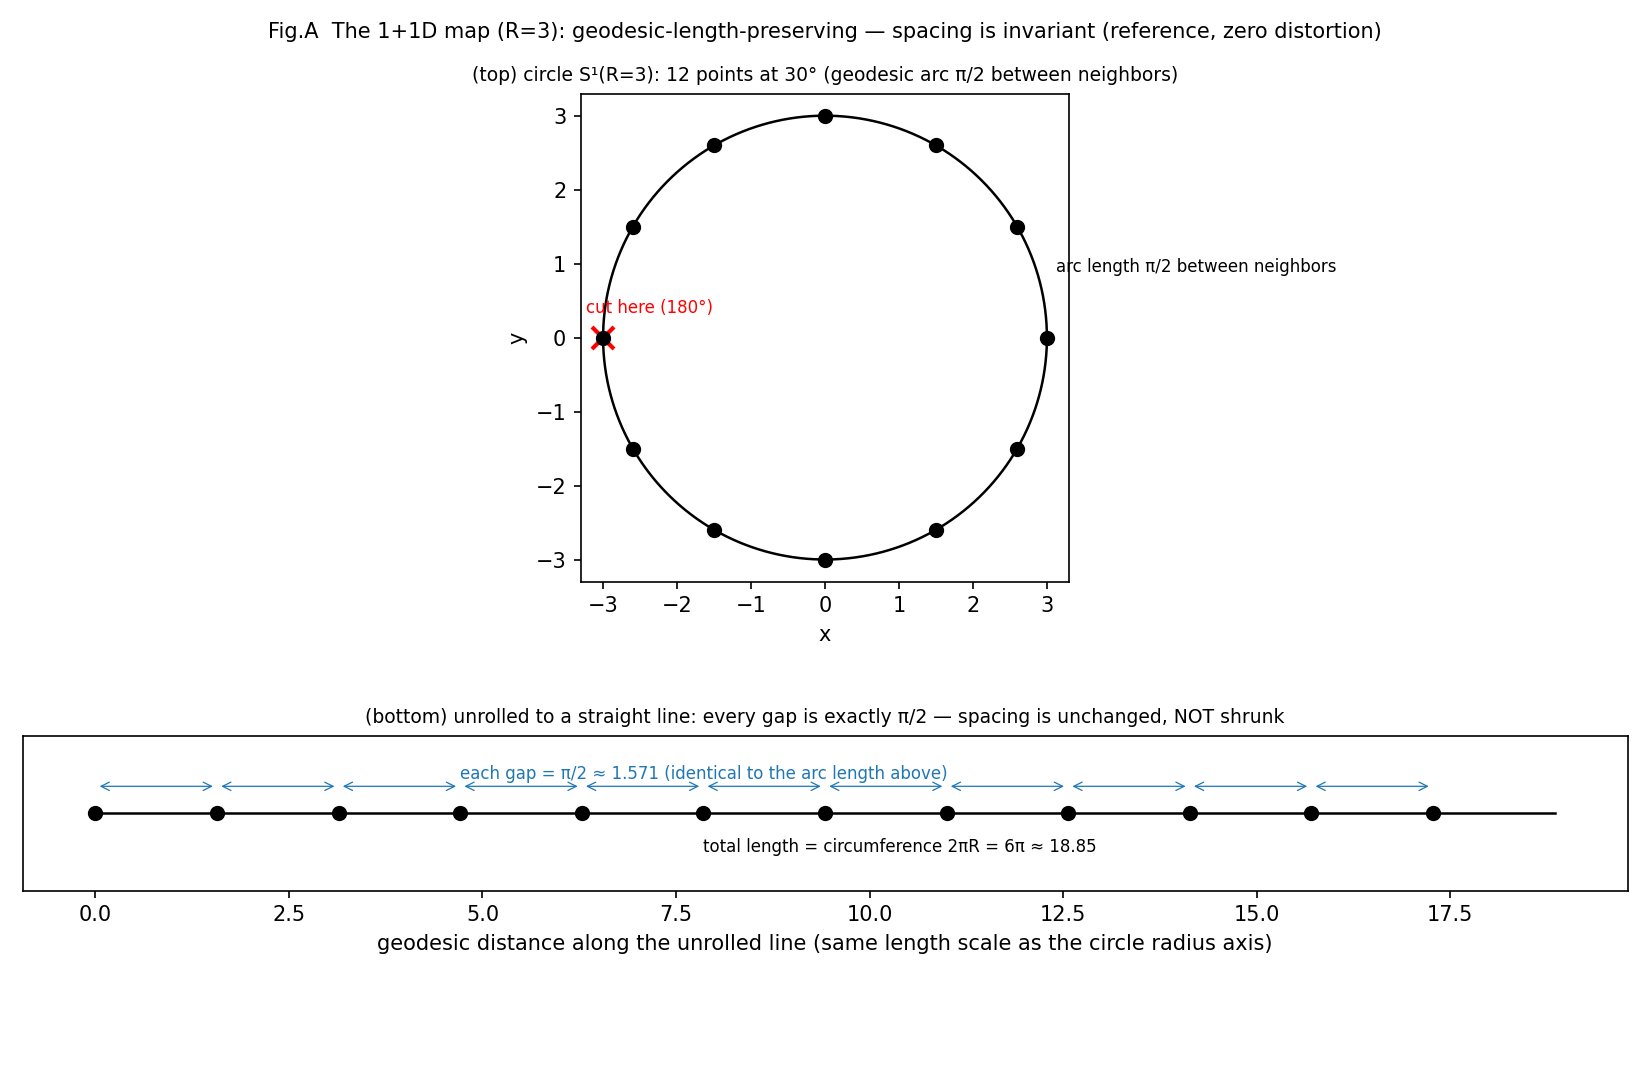
\includegraphics[width=0.88\linewidth,height=\textheight,keepaspectratio]{paper0_figA_1d_reference.png}

\textbf{Fig. A. The 1+1-dimensional map (R=3, reference image)}. Twelve
points at 30° spacing on the circle of radius 3 (geodesic distance π/2
between neighbors). Cutting at 180° and unrolling to a segment, the
spacing stays π/2 --- a geodesic-length-preserving map does not distort
one dimension. All later distortion is read as deviation from this
equal-spacing reference.

\subsection{2. The unified volume formula and the two
dimension-independent
quantities}\label{the-unified-volume-formula-and-the-two-dimension-independent-quantities}

\textbf{Volume (d-content)}: mapping the flat box of the vertex convex
hull by σ\_R, the Jacobian closes (§A),

V\_d(R) = ∫\_\{{[}−t,t{]}\^{}d\} R\^{}d w /
(\textbar y\textbar{}\(^{2}\) + w\(^{2}\))\^{}\{(d+1)/2\} dy. (3)

As R→∞, V\_d→1. For d=2 this matches the Gauss--Bonnet area to machine
precision (difference ≤ 4×10\(^{-14}\)).

\textbf{Vertex angle (distortion of the right angle) ---
dimension-independent}: applying Napier's rule to the spherical right
triangle of center, edge midpoint, and vertex and putting it in closed
form, the angle θ between the two edges meeting at a vertex is

cos θ(R) = −tan\(^{2}\)(1/2R), i.e.~θ(R) = arccos(−tan\(^{2}\)(1/2R)).
(4)

d does not appear in this formula. Numerical computation from tangent
vectors also confirms exact agreement for d=2--5. Flat limit θ→90° ✓;
positive curvature gives θ\textgreater90° ✓. (Equivalent form
sin(θ/2)=1/(√2 cos(1/2R)). Consistent with Gauss--Bonnet.)

\textbf{Area of the 2-face (2-content) --- dimension-independent}: the
2-face is a geodesic square of edge length 1, and by the
\textbf{homogeneity} of the sphere (congruent geodesic squares at any
position have the same area), its area is the same inside a hypercube of
any dimension:

A(R) = V\(_{2}\)(R) = R\(^{2}\)(4θ\_rad − 2π) (equal for all d,
machine-confirmed). (5)

\begin{quote}
\textbf{Organizing the viewpoints (the focus of this version)}: the edge
(1-content), the vertex angle, and the area of the 2-face (2-content)
are all \textbf{intrinsic quantities of dimension ≤2 and do not depend
on dimension}. Dimension d acts only on (i) the \textbf{domain of
existence} (\(R^{*}_{d}\) rises with d) and (ii) the \textbf{volume
(d-content)}.
\end{quote}

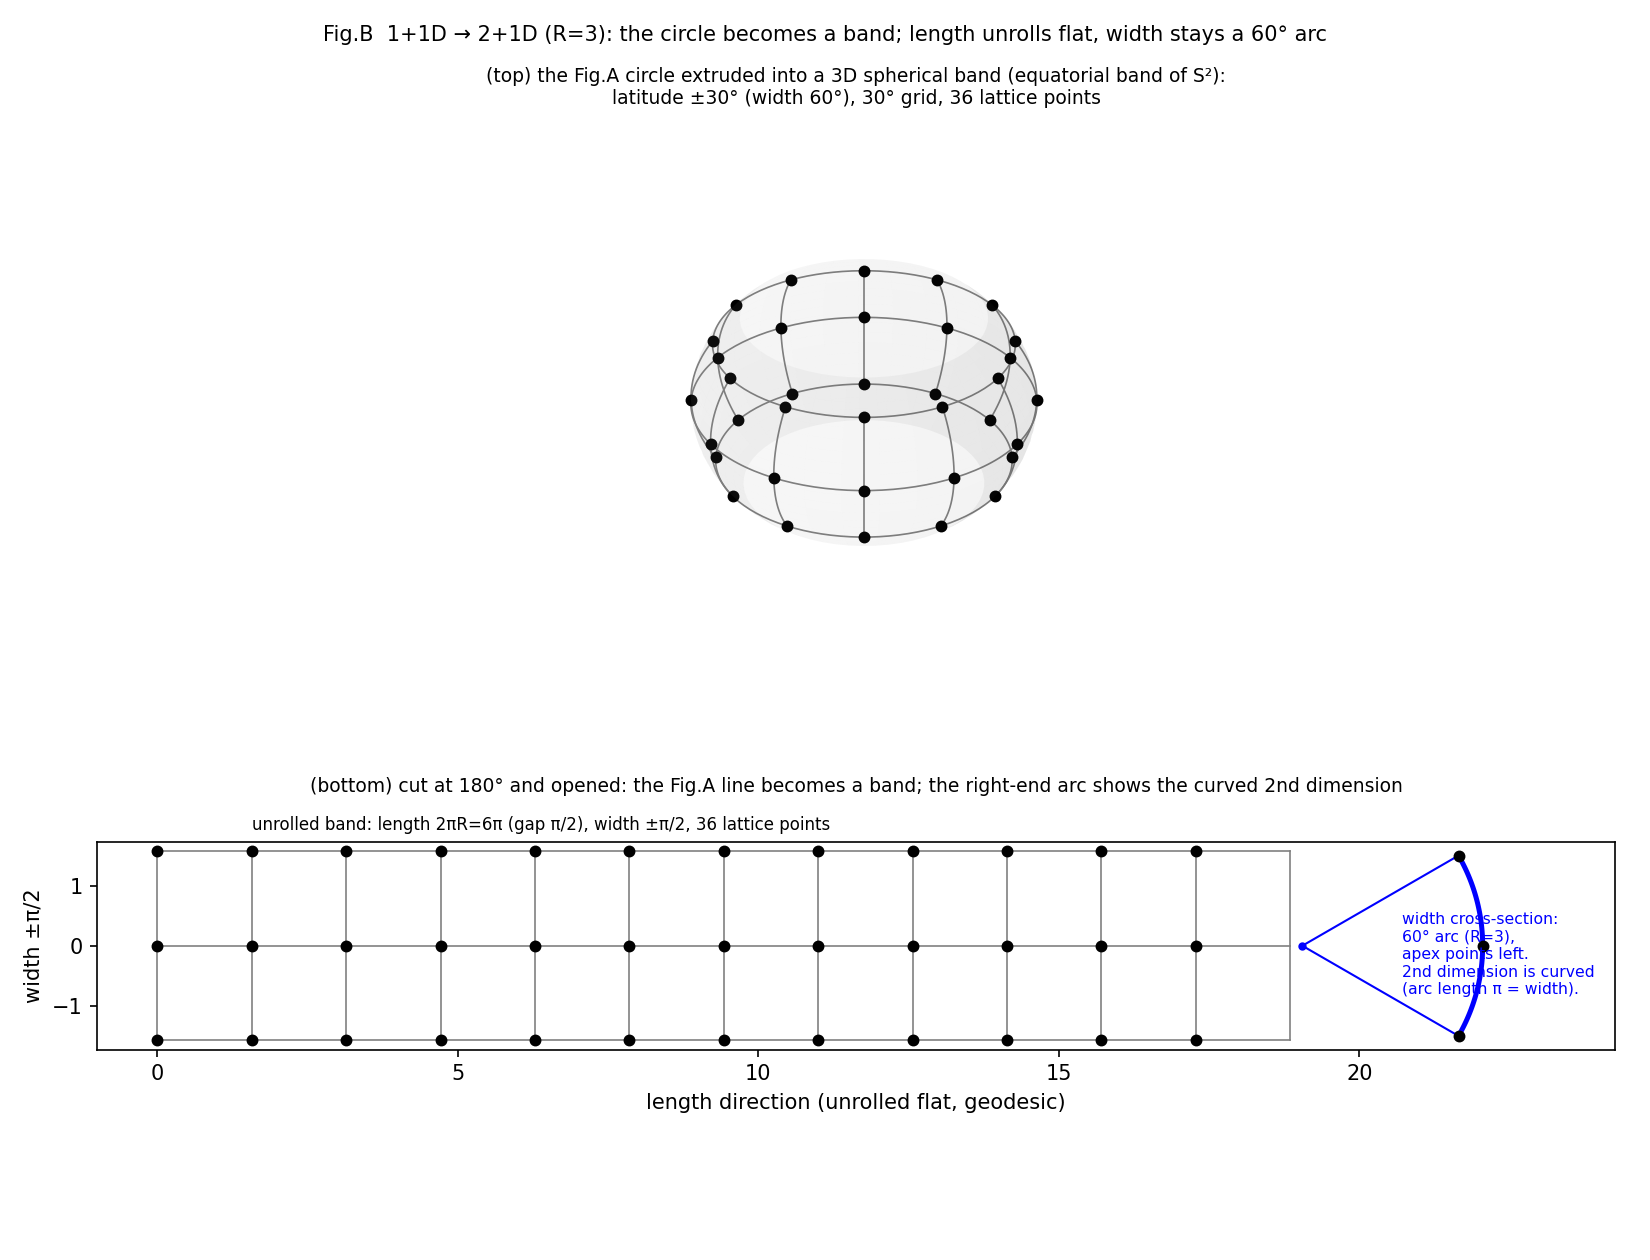
\includegraphics[width=0.88\linewidth,height=\textheight,keepaspectratio]{paper0_figB_band_unfold.png}

\textbf{Fig. B. The 1+1→2+1-dimensional map (R=3, unfolded)}. The circle
of Fig. A extended to a spherical band of latitude ±30° (width 60°)
(top, 30° grid, 36 lattice points). Cutting it open at 180°, the length
direction unrolls into a flat ribbon (bottom), but the width direction
retains curvature as the cross-section of a 60° arc (the fan at the
right end, apex pointing left). Length unrolls flat while width stays
curved --- this asymmetry is the seed of the ``1D→2D'' distortion. The
bulge of this band (height h≈0.102) is the same regardless of dimension
d (§2 dimension-independence).

\subsection{3. The small-angle coefficient of the volume (the only
quantity dimension acts
on)}\label{the-small-angle-coefficient-of-the-volume-the-only-quantity-dimension-acts-on}

Expanding (3) in 1/R, for all dimensions

V\_d(R) = 1 + c\_d/R\(^{2}\) + O(1/R\(^{4}\)), c\_d = d(d−1)/12 =
C(d,2)/6. (6)

Machine verification (R=10\(^{4}\)): for d=2--6, 1/6, 1/2, 1, 5/3, 5/2
--- all in exact agreement with d(d−1)/12. \textbf{Interpretation}: the
volume excess of a d-cube is the \textbf{sum of the area excesses of
each of its C(d,2) coordinate 2-planes (each 1/6=c\(_{2}\))}. The area
excess 1/6 is the ``atom''; the volume is a linear combination of them
(the trace of the curvature 2-form). This is the quantitative form of
§2's ``area is dimension-independent, volume alone is
dimension-dependent.''

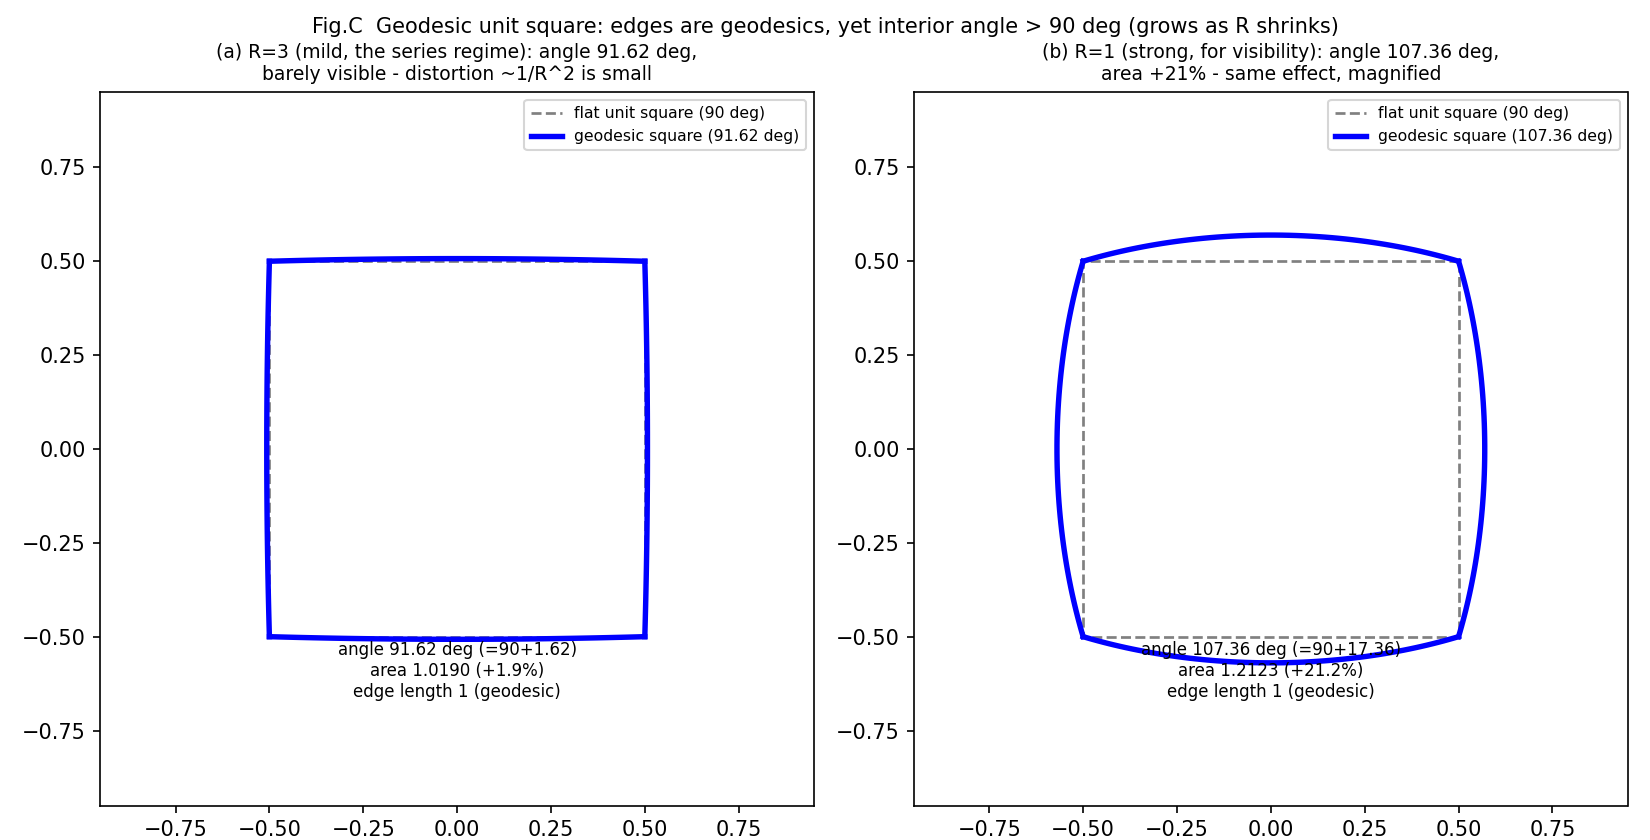
\includegraphics[width=0.88\linewidth,height=\textheight,keepaspectratio]{paper0_figC_angle_excess.png}

\textbf{Fig. C. Angle excess of the geodesic square}. A geodesic square
of edge length 1 (each edge a geodesic = a straight line of that space)
yet its interior angle exceeds 90°. Left: R=3 (the regime of the series,
91.62°, nearly flat, distortion ∝1/R\(^{2}\) is small); right: R=1 (for
visibility, 107.36°, area +21\%, the same effect magnified). The
distortion appears not in edge length but in angle and area, and is
larger the smaller R is.

\subsection{4. Viewpoint tables (machine-computed, fixed
values)}\label{viewpoint-tables-machine-computed-fixed-values}

n/a = below existence threshold (2). ``---'' = the quantity is not
defined for that dimension.

\subsubsection{Table 1: Edge length
(1-content)}\label{table-1-edge-length-1-content}

{\def\LTcaptype{none} % do not increment counter
\begin{longtable}[]{@{}
  >{\raggedright\arraybackslash}p{(\linewidth - 10\tabcolsep) * \real{0.1667}}
  >{\raggedright\arraybackslash}p{(\linewidth - 10\tabcolsep) * \real{0.1667}}
  >{\raggedright\arraybackslash}p{(\linewidth - 10\tabcolsep) * \real{0.1667}}
  >{\raggedright\arraybackslash}p{(\linewidth - 10\tabcolsep) * \real{0.1667}}
  >{\raggedright\arraybackslash}p{(\linewidth - 10\tabcolsep) * \real{0.1667}}
  >{\raggedright\arraybackslash}p{(\linewidth - 10\tabcolsep) * \real{0.1667}}@{}}
\toprule\noalign{}
\begin{minipage}[b]{\linewidth}\raggedright
\end{minipage} & \begin{minipage}[b]{\linewidth}\raggedright
d=1
\end{minipage} & \begin{minipage}[b]{\linewidth}\raggedright
d=2
\end{minipage} & \begin{minipage}[b]{\linewidth}\raggedright
d=3
\end{minipage} & \begin{minipage}[b]{\linewidth}\raggedright
d=4
\end{minipage} & \begin{minipage}[b]{\linewidth}\raggedright
d=5
\end{minipage} \\
\midrule\noalign{}
\endhead
\bottomrule\noalign{}
\endlastfoot
all R (within domain) & 1.000000 & 1.000000 & 1.000000 & 1.000000 &
1.000000 \\
\end{longtable}
}

By geodesic-length preservation, the edge is exactly 1 for all
dimensions, all R (no distortion).

\subsubsection{Table 2: Vertex angle θ {[}deg{]} (distortion from the
right angle 90°) --- equal for
d=2--5}\label{table-2-vertex-angle-ux3b8-deg-distortion-from-the-right-angle-90-equal-for-d25}

{\def\LTcaptype{none} % do not increment counter
\begin{longtable}[]{@{}llllll@{}}
\toprule\noalign{}
R & d=1 & d=2 & d=3 & d=4 & d=5 \\
\midrule\noalign{}
\endhead
\bottomrule\noalign{}
\endlastfoot
0.5 & --- & n/a & n/a & n/a & n/a \\
1.0 & --- & 107.36431 & 107.36431 & 107.36431 & n/a \\
1.5 & --- & 96.88584 & 96.88584 & 96.88584 & 96.88584 \\
2.0 & --- & 93.73831 & 93.73831 & 93.73831 & 93.73831 \\
2.5 & --- & 92.35502 & 92.35502 & 92.35502 & 92.35502 \\
3.0 & --- & 91.62171 & 91.62171 & 91.62171 & 91.62171 \\
3.5 & --- & 91.18548 & 91.18548 & 91.18548 & 91.18548 \\
4.0 & --- & 90.90469 & 90.90469 & 90.90469 & 90.90469 \\
5.0 & --- & 90.57681 & 90.57681 & 90.57681 & 90.57681 \\
6.0 & --- & 90.39974 & 90.39974 & 90.39974 & 90.39974 \\
7.0 & --- & 90.29332 & 90.29332 & 90.29332 & 90.29332 \\
8.0 & --- & 90.22440 & 90.22440 & 90.22440 & 90.22440 \\
9.0 & --- & 90.17720 & 90.17720 & 90.17720 & 90.17720 \\
10.0 & --- & 90.14348 & 90.14348 & 90.14348 & 90.14348 \\
100 & --- & 90.00143 & 90.00143 & 90.00143 & 90.00143 \\
1000 & --- & 90.00001 & 90.00001 & 90.00001 & 90.00001 \\
10000 & --- & 90.00000 & 90.00000 & 90.00000 & 90.00000 \\
\end{longtable}
}

The excess over the right angle Δθ=θ−90° (deg, d-independent): 17.36° at
R=1.0, 6.89° at R=1.5, 3.74° at R=2, 1.62° at R=3, 0.577° at R=5, 0.143°
at R=10, 0.00143° at R=100. Decays as 1/R\(^{2}\).

\subsubsection{Table 3: Area of the 2-face A (2-content) --- equal for
d=2--5
(homogeneity)}\label{table-3-area-of-the-2-face-a-2-content-equal-for-d25-homogeneity}

{\def\LTcaptype{none} % do not increment counter
\begin{longtable}[]{@{}llllll@{}}
\toprule\noalign{}
R & d=1 & d=2 & d=3 & d=4 & d=5 \\
\midrule\noalign{}
\endhead
\bottomrule\noalign{}
\endlastfoot
0.5 & --- & n/a & n/a & n/a & n/a \\
1.0 & --- & 1.2122579 & 1.2122579 & 1.2122579 & n/a \\
1.5 & --- & 1.0816255 & 1.0816255 & 1.0816255 & 1.0816255 \\
2.0 & --- & 1.0439325 & 1.0439325 & 1.0439325 & 1.0439325 \\
2.5 & --- & 1.0275733 & 1.0275733 & 1.0275733 & 1.0275733 \\
3.0 & --- & 1.0189503 & 1.0189503 & 1.0189503 & 1.0189503 \\
4.0 & --- & 1.0105516 & 1.0105516 & 1.0105516 & 1.0105516 \\
5.0 & --- & 1.0067216 & 1.0067216 & 1.0067216 & 1.0067216 \\
6.0 & --- & 1.0046561 & 1.0046561 & 1.0046561 & 1.0046561 \\
7.0 & --- & 1.0034156 & 1.0034156 & 1.0034156 & 1.0034156 \\
8.0 & --- & 1.0026125 & 1.0026125 & 1.0026125 & 1.0026125 \\
9.0 & --- & 1.0020628 & 1.0020628 & 1.0020628 & 1.0020628 \\
10.0 & --- & 1.0016701 & 1.0016701 & 1.0016701 & 1.0016701 \\
100 & --- & 1.0000167 & 1.0000167 & 1.0000167 & 1.0000167 \\
1000 & --- & 1.0000002 & 1.0000002 & 1.0000002 & 1.0000002 \\
10000 & --- & 1.0000000 & 1.0000000 & 1.0000000 & 1.0000000 \\
\end{longtable}
}

The excess over the flat unit square (area 1) is A−1 ≈ 1/(6R\(^{2}\)).
About +1.9\% at R=3.

\subsubsection{Table 4: Volume V\_d (d-content) --- the only quantity
that genuinely differs by
dimension}\label{table-4-volume-v_d-d-content-the-only-quantity-that-genuinely-differs-by-dimension}

{\def\LTcaptype{none} % do not increment counter
\begin{longtable}[]{@{}llllll@{}}
\toprule\noalign{}
R & d=1 & d=2 & d=3 & d=4 & d=5 \\
\midrule\noalign{}
\endhead
\bottomrule\noalign{}
\endlastfoot
0.5 & 1.000000 & n/a & n/a & n/a & n/a \\
1.0 & 1.000000 & 1.2122579 & 1.9499111 & 5.4161376 & n/a \\
1.5 & 1.000000 & 1.0816255 & 1.2801348 & 1.6834544 & 2.5128373 \\
2.0 & 1.000000 & 1.0439325 & 1.1413925 & 1.3119759 & 1.5924206 \\
2.5 & 1.000000 & 1.0275733 & 1.0864041 & 1.1834234 & 1.3302164 \\
3.0 & 1.000000 & 1.0189503 & 1.0585685 & 1.1219513 & 1.2139814 \\
3.5 & 1.000000 & 1.0138368 & 1.0424191 & 1.0873448 & 1.1510492 \\
4.0 & 1.000000 & 1.0105516 & 1.0321808 & 1.0657975 & 1.1127589 \\
4.5 & 1.000000 & 1.0083144 & 1.0252687 & 1.0514201 & 1.0875871 \\
5.0 & 1.000000 & 1.0067216 & 1.0203771 & 1.0413269 & 1.0700953 \\
6.0 & 1.000000 & 1.0046561 & 1.0140697 & 1.0284116 & 1.0479269 \\
7.0 & 1.000000 & 1.0034156 & 1.0103013 & 1.0207484 & 1.0348864 \\
8.0 & 1.000000 & 1.0026125 & 1.0078694 & 1.0158237 & 1.0265506 \\
9.0 & 1.000000 & 1.0020628 & 1.0062083 & 1.0124694 & 1.0208927 \\
10.0 & 1.000000 & 1.0016701 & 1.0050232 & 1.0100810 & 1.0168738 \\
100 & 1.000000 & 1.0000167 & 1.0000500 & 1.0001000 & 1.0001667 \\
1000 & 1.000000 & 1.0000002 & 1.0000005 & 1.0000010 & 1.0000017 \\
10000 & 1.000000 & 1.0000000 & 1.0000000 & 1.0000000 & 1.0000000 \\
\end{longtable}
}

(d=1 is a segment = locally flat, V\(_{1}\)=1. For d≥2 the excess is
c\_d/R\(^{2}\), c\_d=1/6, 1/2, 1, 5/3.)

\textbf{Limit verification (passes)}: at R=100/1000/10000 all quantities
decay to the flat value as 1/R\(^{2}\) (factor 100\(^{2}\) each step).
For all R, V\_d\textgreater1, θ\textgreater90° (monotone
positive-curvature excess).

\subsection{4.5 Inverting curvature from the angle --- the internal
observer's curvature
meter}\label{inverting-curvature-from-the-angle-the-internal-observers-curvature-meter}

In §2 the vertex angle is the dimension-independent quantity cos
θ=−tan\(^{2}\)(1/2R), and as Table 2 (§4) shows it is equal for d=2--5.
An important consequence follows: \textbf{if d≥2, the angle can be
measured, and from it the curvature radius R (more essentially the
curvature K=1/R\(^{2}\)) can be inverted}. This means that for an
internal observer (one who cannot see the embedding), the
\textbf{``direction'' of curvature is unknowable but its ``value'' is
knowable}.

\subsubsection{Extension to negative
curvature}\label{extension-to-negative-curvature}

As the analytic continuation of the sphere (positive curvature
K=+1/R\(^{2}\)), in hyperbolic space (negative curvature K=−1/R\(^{2}\))
sin→sinh, and from a tangent-vector computation in the hyperboloid model
(Minkowski metric)

cos θ(R) = +tanh\(^{2}\)(1/2R) (negative curvature, θ \textless{} 90°,
dimension-independent for all d, machine-confirmed). (8)

\textbf{Positive--negative asymmetry (remark A)}: in hyperbolic space
t=R sinh(1/2R), w=R√(1+d sinh\(^{2}\)(1/2R)), and the radicand is always
positive --- \textbf{a cell of edge length 1 has no existence threshold
and is constructible for all R, all d} (machine-confirmed). This
contrasts with positive curvature, where at \(R^{*}_{d}\)=1/(2
arcsin(1/√d)) the cell reaches the equator and vanishes (§1 (2)). The
negative-curvature table (θ=84°→R=1.49 etc.) is defined everywhere under
this thresholdlessness.

Placed alongside positive curvature (4), \textbf{the sign of the vertex
angle determines the sign of curvature}:

{\def\LTcaptype{none} % do not increment counter
\begin{longtable}[]{@{}
  >{\raggedright\arraybackslash}p{(\linewidth - 6\tabcolsep) * \real{0.2500}}
  >{\raggedright\arraybackslash}p{(\linewidth - 6\tabcolsep) * \real{0.2500}}
  >{\raggedright\arraybackslash}p{(\linewidth - 6\tabcolsep) * \real{0.2500}}
  >{\raggedright\arraybackslash}p{(\linewidth - 6\tabcolsep) * \real{0.2500}}@{}}
\toprule\noalign{}
\begin{minipage}[b]{\linewidth}\raggedright
Vertex angle
\end{minipage} & \begin{minipage}[b]{\linewidth}\raggedright
Curvature
\end{minipage} & \begin{minipage}[b]{\linewidth}\raggedright
Space
\end{minipage} & \begin{minipage}[b]{\linewidth}\raggedright
Relation
\end{minipage} \\
\midrule\noalign{}
\endhead
\bottomrule\noalign{}
\endlastfoot
θ \textgreater{} 90° (excess over right angle) & K \textgreater{} 0 &
spherical & cos θ = −tan\(^{2}\)(1/2R) \\
θ = 90° (right angle) & K = 0 & flat & --- \\
θ \textless{} 90° (deficit from right angle) & K \textless{} 0 &
hyperbolic & cos θ = +tanh\(^{2}\)(1/2R) \\
\end{longtable}
}

That is, \textbf{if the angle is less than 90°, the curvature is
negative}. The sign of the deviation Δθ=θ−90° from the right angle is
exactly the sign of curvature.

\subsubsection{Inversion formula (curvature
meter)}\label{inversion-formula-curvature-meter}

Normalizing the edge to unit a=1, from the measured vertex angle θ the
curvature and radius are uniquely recovered:

θ \textgreater{} 90°: R = 1/(2 arctan√(−cos θ)), K = +1/R\(^{2}\) θ
\textless{} 90°: R = 1/(2 artanh√(+cos θ)), K = −1/R\(^{2}\) (9)

The round-trip check (R→θ→inverted R) agrees to machine precision for
both positive and negative curvature, R=1.5--100. Numerical examples of
the inversion:

{\def\LTcaptype{none} % do not increment counter
\begin{longtable}[]{@{}llll@{}}
\toprule\noalign{}
measured θ {[}deg{]} & curvature K & radius R & type \\
\midrule\noalign{}
\endhead
\bottomrule\noalign{}
\endlastfoot
84.0 & −0.449805 & 1.49103 & negative (hyperbolic) \\
88.0 & −0.142935 & 2.64503 & negative (hyperbolic) \\
89.5 & −0.035111 & 5.33680 & negative (hyperbolic) \\
90.0 & 0 & ∞ & flat \\
90.5 & +0.034704 & 5.36794 & positive (spherical) \\
92.0 & +0.136435 & 2.70731 & positive (spherical) \\
96.0 & +0.391129 & 1.59897 & positive (spherical) \\
107.36431 & +1.000000 & 1.00000 & positive (spherical) \\
\end{longtable}
}

\subsubsection{Meaning (connection to the theme of the
series)}\label{meaning-connection-to-the-theme-of-the-series}

\begin{enumerate}
\def\labelenumi{(\roman{enumi})}
\item
  \textbf{Dimensional universality}: the inversion formula (9) contains
  no d.~A 2-dimensional observer and a 4-dimensional observer obtain
  \textbf{the same K} by measuring the local vertex angle --- the
  curvature meter does not care about dimension.
\item
  \textbf{Direction invisible, value knowable}: the internal observer
  cannot know the ``orientation'' of curvature (which way it bends in
  the embedding, the pole position = marking). That is a gauge (an
  invisible direction). But the curvature scalar K (sign and magnitude)
  is fully determined from \textbf{a single local angle measurement}.
  This is isomorphic to the schema in the main series where R and Q are
  invariants shared by all markings while which axis is time (the
  orientation) is gauge (Paper 14 marking theorem).
\item
  \textbf{It cannot be measured at d=1}: one dimension has no vertex
  angle (only edges), and the curvature meter requires d≥2. This is the
  observational side of ``distortion first arises at d≥2'' (its first
  basis is §1--2: d=1 is intrinsically flat with zero distortion; the
  summary is in §7).
\end{enumerate}

\subsection{4.6 Dimensional ambiguity and the conjugate quantity of
dimension
(observation)}\label{dimensional-ambiguity-and-the-conjugate-quantity-of-dimension-observation}

Solving §1's existence condition d·sin\(^{2}\)(1/2R) ≤ 1 \textbf{for
dimension} gives the \textbf{maximum dimension} in which a regular
geodesic cell of edge length 1 fits at a given curvature radius R:

\(d_{\max}(R) = \lfloor 1/\sin^2(1/2R)\rfloor = \lfloor \csc^2(1/2R)\rfloor \approx 4R^2\)
(large-R asymptotics), \(R \ge 1/\pi\). (10)

That is, \textbf{dimension is bounded from above by curvature}. The
allowed dimensions lie in the range \{1, 2, \ldots, d\_max(R)\} and are
not uniquely determined --- \textbf{for a given R, dimension has
ambiguity}.

\subsubsection{Dimensional ambiguity (relatively) increases at small
R}\label{dimensional-ambiguity-relatively-increases-at-small-r}

Propagating the uncertainty ±½ in R (§6), the ceiling d\_max itself
acquires a width:

{\def\LTcaptype{none} % do not increment counter
\begin{longtable}[]{@{}
  >{\raggedright\arraybackslash}p{(\linewidth - 10\tabcolsep) * \real{0.1667}}
  >{\raggedright\arraybackslash}p{(\linewidth - 10\tabcolsep) * \real{0.1667}}
  >{\raggedright\arraybackslash}p{(\linewidth - 10\tabcolsep) * \real{0.1667}}
  >{\raggedright\arraybackslash}p{(\linewidth - 10\tabcolsep) * \real{0.1667}}
  >{\raggedright\arraybackslash}p{(\linewidth - 10\tabcolsep) * \real{0.1667}}
  >{\raggedright\arraybackslash}p{(\linewidth - 10\tabcolsep) * \real{0.1667}}@{}}
\toprule\noalign{}
\begin{minipage}[b]{\linewidth}\raggedright
R
\end{minipage} & \begin{minipage}[b]{\linewidth}\raggedright
κ=sin\(^{2}\)(1/2R)
\end{minipage} & \begin{minipage}[b]{\linewidth}\raggedright
d\_max(R−½)
\end{minipage} & \begin{minipage}[b]{\linewidth}\raggedright
d\_max(R)
\end{minipage} & \begin{minipage}[b]{\linewidth}\raggedright
d\_max(R+½)
\end{minipage} & \begin{minipage}[b]{\linewidth}\raggedright
relative width Δd/d
\end{minipage} \\
\midrule\noalign{}
\endhead
\bottomrule\noalign{}
\endlastfoot
0.5 & 0.708073 & 0 & 1 & 4 & 3.000 \\
0.7 & 0.429127 & 0 & 2 & 6 & 2.500 \\
1.0 & 0.229849 & 1 & 4 & 9 & 2.000 \\
1.5 & 0.107056 & 4 & 9 & 16 & 1.333 \\
2.0 & 0.061209 & 9 & 16 & 25 & 1.000 \\
3.0 & 0.027522 & 25 & 36 & 49 & 0.667 \\
5.0 & 0.009967 & 81 & 100 & 121 & 0.400 \\
10.0 & 0.002498 & 361 & 400 & 441 & 0.200 \\
\end{longtable}
}

(d\_max=0 for R\textless1/π≈0.318 is the pre-geometric region = a point
with no structure, unified with §4.7.)

\textbf{The relative dimensional ambiguity Δd/d is larger the smaller R
is} (at R=1, d\_max swings 1--9). In the small-R region ±½ is relatively
huge, so dimension is not sharply determined. Conversely at large R
(near flat) the ceiling is high (d\_max≈4R\(^{2}\)) but the relative
width shrinks as 1/R and dimension stabilizes. Two readings coexist:
\textbf{strong curvature lowers the absolute ceiling (restricting
dimension to low values) and at the same time raises the relative
ambiguity under the ±½ fluctuation}.

\subsubsection{Candidate for the conjugate quantity of
dimension}\label{candidate-for-the-conjugate-quantity-of-dimension}

\begin{enumerate}
\def\labelenumi{(\arabic{enumi})}
\setcounter{enumi}{9}
\tightlist
\item
  can be written as the capacity relation \textbf{d·κ ≤ 1} (κ ≡
  sin\(^{2}\)(1/2R), budget 1). Saturation d·κ=1 is exactly the ceiling
  \(R^{*}_{d}\) (10-digit agreement confirmed for d=2--5). The remaining
  capacity is geometrically
\end{enumerate}

1 − d·κ = (w/R)\(^{2}\) (the cosine\(^{2}\) of the polar colatitude of
the cell center; 0 when the vertices reach the equator).

That is, \textbf{each spatial dimension consumes κ from the unit
curvature budget, and reaches the dimensional ceiling when the budget is
exhausted}. In the large-R asymptotics κ ≈ 1/(4R\(^{2}\)) = K/4
(K=1/R\(^{2}\) is curvature), and

d × (K/4) ≲ 1, i.e.~dimension ≲ 4/curvature.

(Bridge: K=1/R\(^{2}\) so 4/K=4R\(^{2}\). Thus ``d\_max≈4R\(^{2}\)
(large R, top of §4.6)'' and ``d·(K/4)≲1'' are two notations for the
same relation.)

\begin{quote}
\textbf{Observation (a problem statement, not a claim of this paper)}:
the geometric candidate for the designer's question ``what is the
conjugate quantity of dimension'' is \textbf{the per-axis curvature load
κ=sin\(^{2}\)(1/2R) (≈ curvature/4)}. Dimension d and κ form a capacity
conjugate pair (d·κ≤1), in the same ``saturation of a conserved budget''
relation as νλ=1 and Σν\(^{2}\)=\(\mathcal{N}\)\(^{2}\) (Paper 1). This
is an exact geometric fact (a restatement of the existence condition),
but its \textbf{interpretation as conjugacy is an observation, not a
theorem}. No physical identification is made.
\end{quote}

\subsubsection{Implication for the series (explicit
scope)}\label{implication-for-the-series-explicit-scope}

The R at which this series operates is small (R=1--3 or so). There, by
(10), d\_max=4--36, and \textbf{dimension 4 is just one value
geometrically allowed; geometry alone does not fix d=4}. The fixing to
d=4 is due to the arithmetic mechanism of Paper 11
(\{1,2,4,8\}∩squares), which is a separate axis from the geometric
ambiguity here. What this paper shows is the fact, complementary to
Paper 11, that ``geometry gives dimension a ceiling and an ambiguity,
but does not select a particular dimension.'' \textbf{A full connection
to the discrete system (a formulation of a dimensional uncertainty
relation) is outside the scope of this paper and is left as an
observation.}

\subsubsection{Relation to prior work
(differentiation)}\label{relation-to-prior-work-differentiation}

The idea that dimension need not be unique and can depend on scale is
not itself new. The \textbf{spectral dimension} measured by diffusion is
known to flow from ∼2 at short distances to ∼4 at long distances in
quantum gravity (causal dynamical triangulations, asymptotic safety,
loop quantum gravity) {[}Carlip 2017; Ambjørn--Jurkiewicz--Loll 2005{]},
and dimensional regularization and fractal dimension are of the same
family. In a constant-curvature space, the closest precedent for a
\textbf{curvature-radius-dependent geometric bound} is the
\textbf{Böröczky packing-density upper bound} {[}Böröczky 1978{]}. This
paper differs in three respects: (i) the source of the ceiling is not
diffusion or density but a \textbf{discrete existence condition}
d·sin\(^{2}\)(1/2R)≤1 --- ``do integer-many regular geodesic cells of
edge 1 fit?'' (the existence threshold \(R^{*}_{d}\) belongs to the
lineage of the Schläfli-type existence condition for regular spherical
polytopes {[}Coxeter 1973{]}); (ii) this takes the form of a
\textbf{conjugate quantity of dimension} κ=sin\(^{2}\)(1/2R) with a
capacity relation d·κ≤1, lying on the same
saturation-of-a-conserved-budget pattern as νλ=1 and
Σν\(^{2}\)=\(\mathcal{N}\)\(^{2}\); (iii) the geometric ceiling and the
censorship ceiling of Paper 11 are \textbf{two independent mechanisms
that critically coincide at d=4} (§4.7). ``Why four dimensions'' has
long been argued in many ways {[}Ehrenfest 1917; Tegmark 1997{]}, but
the claim of this paper lies in the \textbf{specificity of this chain},
not in advancing ``dimensional ambiguity'' in general as a new concept.

\subsection{4.7 Emergence of dimension from zero and stabilization at
d=4
(observation)}\label{emergence-of-dimension-from-zero-and-stabilization-at-d4-observation}

The geometric ceiling d\_max(R)≈4R\(^{2}\) of §4.6 \textbf{rises with R}
(as curvature weakens, higher dimensions fit). Overlaying Paper 11's
\textbf{censorship ceiling}, the emergence of dimension and its
stabilization at d=4 become a single picture.

\subsubsection{The two ceilings}\label{the-two-ceilings}

\begin{itemize}
\tightlist
\item
  \textbf{Geometric ceiling (this paper)}:
  d\_max(R)=\(\lfloor\)csc\(^{2}\)(1/2R)\(\rfloor\)≈4R\(^{2}\). Lower
  the smaller R (stronger curvature), rising with R.
\item
  \textbf{Censorship ceiling (Paper 11 both-endpoints theorem; Appendix
  25--26)}: the ladder curvature distortion (√d−1)\(^{2}\)/2
  (\textbf{this formula is derived in Paper 11; this paper uses it as
  given} --- the ladder comes from the diagonal √d of the dressed
  frequency, the half-wavelength censorship bound ½ is Paper 9) is ≤ ½
  only for d ≤ 4. \textbf{d=4 is exactly the equality (√4−1)\(^{2}\)/2=½
  (critical)}; at d=5 it is 0.764\textgreater½, censored and unstable.
  This ceiling is \textbf{fixed at 4}, independent of R.
\end{itemize}

The dimension that can exist stably is the smaller of the two ceilings,
\textbf{d\_stable(R)=min(d\_max(R), 4)}.

\subsubsection{The dimensional staircase
(machine-computed)}\label{the-dimensional-staircase-machine-computed}

{\def\LTcaptype{none} % do not increment counter
\begin{longtable}[]{@{}
  >{\raggedright\arraybackslash}p{(\linewidth - 6\tabcolsep) * \real{0.2500}}
  >{\raggedright\arraybackslash}p{(\linewidth - 6\tabcolsep) * \real{0.2500}}
  >{\raggedright\arraybackslash}p{(\linewidth - 6\tabcolsep) * \real{0.2500}}
  >{\raggedright\arraybackslash}p{(\linewidth - 6\tabcolsep) * \real{0.2500}}@{}}
\toprule\noalign{}
\begin{minipage}[b]{\linewidth}\raggedright
range of R
\end{minipage} & \begin{minipage}[b]{\linewidth}\raggedright
geometric ceiling d\_max
\end{minipage} & \begin{minipage}[b]{\linewidth}\raggedright
stable dimension d\_stable
\end{minipage} & \begin{minipage}[b]{\linewidth}\raggedright
state
\end{minipage} \\
\midrule\noalign{}
\endhead
\bottomrule\noalign{}
\endlastfoot
R \textless{} 1/π≈0.318 & 0 & 0 & pre-geometric (point) \\
{[}1/π, 2/π) & 1 & 1 & d=1 \\
{[}2/π, \(R^{*}_{3}\))≈{[}0.637, 0.812) & 2 & 2 & d=2 \\
{[}\(R^{*}_{3}\), 3/π)≈{[}0.812, 0.955) & 3 & 3 & d=3 \\
\textbf{R ≥ 3/π≈0.955} & 4, 9, 16, \ldots{} (rising) & \textbf{4 (lock)}
& \textbf{censorship caps at 4} \\
\end{longtable}
}

The emergence threshold of each dimension is exactly the
\(R^{*}_{d}\)=1/(2 arcsin(1/√d)) of §1 (2): d=k emerges geometrically at
R≥\(R^{*}_{k}\).

\subsubsection{The narrative: climb, then lock at
4}\label{the-narrative-climb-then-lock-at-4}

\begin{enumerate}
\def\labelenumi{(\roman{enumi})}
\item
  \textbf{From zero dimension}: at strongest curvature (smallest R) the
  geometric ceiling is low and dimension is held to 0--1 (starting from
  a structureless point/segment).
\item
  \textbf{Emergence of dimension (climbing the staircase)}: as R
  increases (curvature weakens = can correspond to the internal
  expansion a∝√t of Paper 8) the geometric ceiling d\_max rises.
  \textbf{But what emerges (is realized) is the stable dimension
  d\_stable=min(d\_max, 4); d\_max itself is merely the monotonically
  rising upper bound on ``the maximum dimension that could fit''}
  (d\_max(3)=36, yet realization is 4 at the censorship ceiling). That
  d\_stable climbs d=1→2→3→4 one step at a time is the emergence, and
  the ±½ makes it not a sharp jump but a fuzzy step (§4.6).
\item
  \textbf{Why it stops at 4}: at R=3/π the rising geometric ceiling
  reaches exactly the fixed censorship ceiling 4. If R increases
  further, geometrically d=5,6,\ldots{} would also fit (d\_max→∞), but
  they are \textbf{unstable} with censorship distortion
  (√d−1)\(^{2}\)/2\textgreater½ (Paper 11). Thus the stable dimension is
  locked at 4 and stays 4 no matter how much it expands afterward.
\end{enumerate}

\begin{quote}
\textbf{Observation (a synthesis, not a claim of this paper)}:
\textbf{d=4 is the unique dimension where the rising geometric ceiling
and the fixed censorship ceiling cross --- the last step that is both
reachable and stable}. Moreover d=4 is the \textbf{critical} point where
the censorship distortion is exactly ½ (equality), and is selected as
``the maximal yet marginally stable'' dimension. The picture in which
dimension emerges with expansion from zero and stabilizes at 4 is
obtained as the \textbf{composition of two independent mechanisms} ---
the geometric ceiling of this paper (§4.6) and the censorship ceiling of
Paper 11. This is a synthesis of two exact facts, not a claim about the
emergence as a physical process. No physical identification is made.
\end{quote}

\subsubsection{Explicit scope}\label{explicit-scope}

What this paper newly provides is the single fact ``the geometric
ceiling rises with R''; the privilege of d=4 and the ladder-distortion
formula (√d−1)\(^{2}\)/2 are borne by Paper 11 (both-endpoints theorem,
Appendix 25--26), which this paper composes as given. The two are
independent (one the geometry of curvature radius, the other the
integrality and censorship of the ladder), and their coincidence lends
the picture its force. Formulating the dynamics of the expansion R(t)
and the time evolution of dimensional emergence is outside the scope of
this paper and left as an observation.

\subsection{4.8 Curvature-exactness of the 1-dimensional logic wave and
the connection to Paper 9
(observation)}\label{curvature-exactness-of-the-1-dimensional-logic-wave-and-the-connection-to-paper-9-observation}

The first result of this paper (§2) was that \textbf{the d=1 geodesic
cell is intrinsically flat --- edge, angle, area, and volume all have
zero distortion, independent of R (including R=3)}. We make explicit how
this bears on the foundation of the main series.

\subsubsection{The waves of the series are 1-dimensional per
axis}\label{the-waves-of-the-series-are-1-dimensional-per-axis}

The dictionary theorem of Paper 5 identified the wave nature of the
count N\(_{0}\)(R) as a \textbf{product of real Fourier bases} with a
zero shift +½ added to each axis's frequency m\(_i\) (the per-axis
multiplicity pattern \{1,2,2,\ldots\} is exactly the real Fourier
basis). That is, \textbf{the content of the wave is a product of
per-axis 1-dimensional standing waves}. The count of Paper 2 is the
integer lattice count of flat 4-cells of edge 1 (each volume
1\(^{4}\)=1), not a measure on a curved surface. The logic wave of Paper
9 §2.1 (the odd-harmonic series of the zero-shift ½ basis, square wave,
position=phase, translation=linear phase multiplication) is also a
per-axis 1-dimensional, longitudinal-type structure.

\subsubsection{Two independent grounds reach the same
conclusion}\label{two-independent-grounds-reach-the-same-conclusion}

The designer's claim ``even with R small (e.g.~R=3), if a 1-dimensional
wave can neglect amplitude (handle amplitude canonically =
longitudinally, as a square wave / logic wave), it is exact'' is
supported by \textbf{two independent routes}:

\begin{itemize}
\tightlist
\item
  \textbf{Geometry (this paper §2)}: a per-axis 1-dimensional wave lives
  at d=1. The curvature distortion at d=1 is \textbf{exactly zero} (any
  R). Hence the flat treatment of a 1-dimensional wave is exact, not
  approximate.
\item
  \textbf{Energy (Paper 9 §2.3 ``curvature consistency'')}: Paper 9 §2.3
  states ``amplitude is displacement out of the propagation direction,
  and its square's local energy density couples with local curvature to
  self-interact. A phase-only wave (±1 values) has uniform local energy
  density, and the linear phase computation survives exactly'' (the
  quotation is the gist of Paper 9 §2.3; this paper places it as given
  alongside the geometric side d=1=0).
\end{itemize}

Geometry (d=1 = zero distortion) and energy (no amplitude = no curvature
coupling) are different reasonings, but \textbf{the curvature-exactness
of the same object (an amplitude-free 1-dimensional logic wave) is
confirmed consistently from two sides} (two sides of the same object,
not a coincidental agreement of two independent propositions). Paper 0
gives this convergence the \textbf{quantitative, geometric ground} for
what Paper 9 stated qualitatively as ``curvature consistency'' (c\_d=0
at d=1; first c\_d=d(d−1)/12\textgreater0 at d≥2).

\subsubsection{The non-uniqueness of reading is another expression of
the §4.6 dimensional
ambiguity}\label{the-non-uniqueness-of-reading-is-another-expression-of-the-4.6-dimensional-ambiguity}

Note that \textbf{the same N\(_{0}\)(R) cell can be read in two ways}:
the per-axis 1-dimensional reading (c\(_{1}\)=0, no correction), and the
d-dimensional coupled reading (c\_d\textgreater0, e.g.~12\% excess at
d=4). Which reading is correct is not settled by Paper 0 alone --- this
is not a defect but \textbf{another expression of the ``dimensional
ambiguity'' of §4.6}: the per-axis 1-dimensional reading and the
d-dimensional coupled reading of the same cell are two compatible
projections, and which one is taken corresponds to the dimensional
ambiguity. The series adopts the former (flat lattice + per-axis
1-dimensional, Papers 2/5/9) by construction. This paper does not
justify the choice; it makes explicit that the two readings coexist and
which one the series takes.

\subsubsection{Implication: the seat of distortion is d≥2, and the logic
wave avoids
it}\label{implication-the-seat-of-distortion-is-d2-and-the-logic-wave-avoids-it}

The distortion of §3--4 (c\_d\textgreater0) appears only in \textbf{true
geodesic cells at d≥2 (coupled geometry with vertex angles)}. By
treating the count with a flat lattice (Paper 2), the wave per-axis
1-dimensionally (Paper 5), and the amplitude canonically (Paper 9), the
series \textbf{avoids the seat of distortion (coupled geometry at d≥2)
by construction and stays in the curvature-exact region}. This is the
geometric backing of the designer's claim, and at the same time the
precise statement of ``what Paper 0 means for the series'':
\textbf{Paper 0 does not supplement a deficiency of the flat treatment;
it demarcates the range in which the flat treatment is exactly valid,
and shows that it coincides with the range where the logic wave lives}.
No physical identification is made.

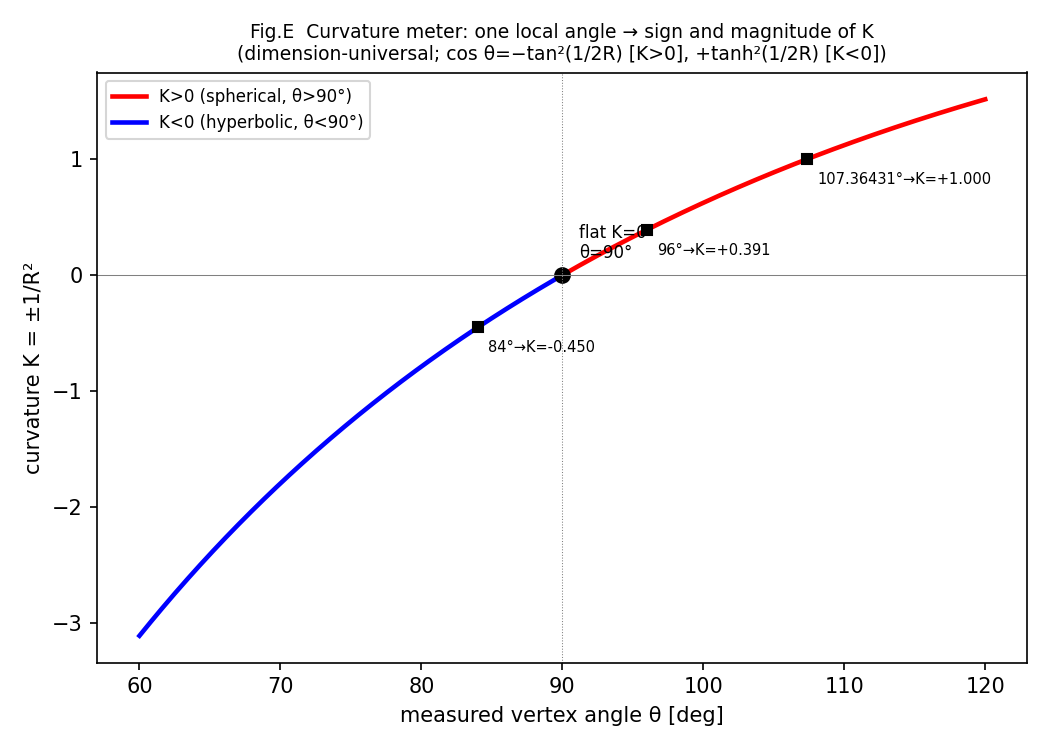
\includegraphics[width=0.88\linewidth,height=\textheight,keepaspectratio]{paper0_figE_curvature_meter.png}

\textbf{Fig. E. The curvature meter (§4.5)}. A single curve that inverts
the curvature K from the measured vertex angle θ. θ\textless90° gives
K\textless0 (hyperbolic), θ=90° gives K=0 (flat), θ\textgreater90° gives
K\textgreater0 (spherical). The inversion examples (84°→K=−0.45, etc.)
lie on the curve. The formula contains no d and is dimension-universal
--- the internal observer cannot know the direction of curvature (the
marking), but can read the sign and magnitude of K from a single local
angle.

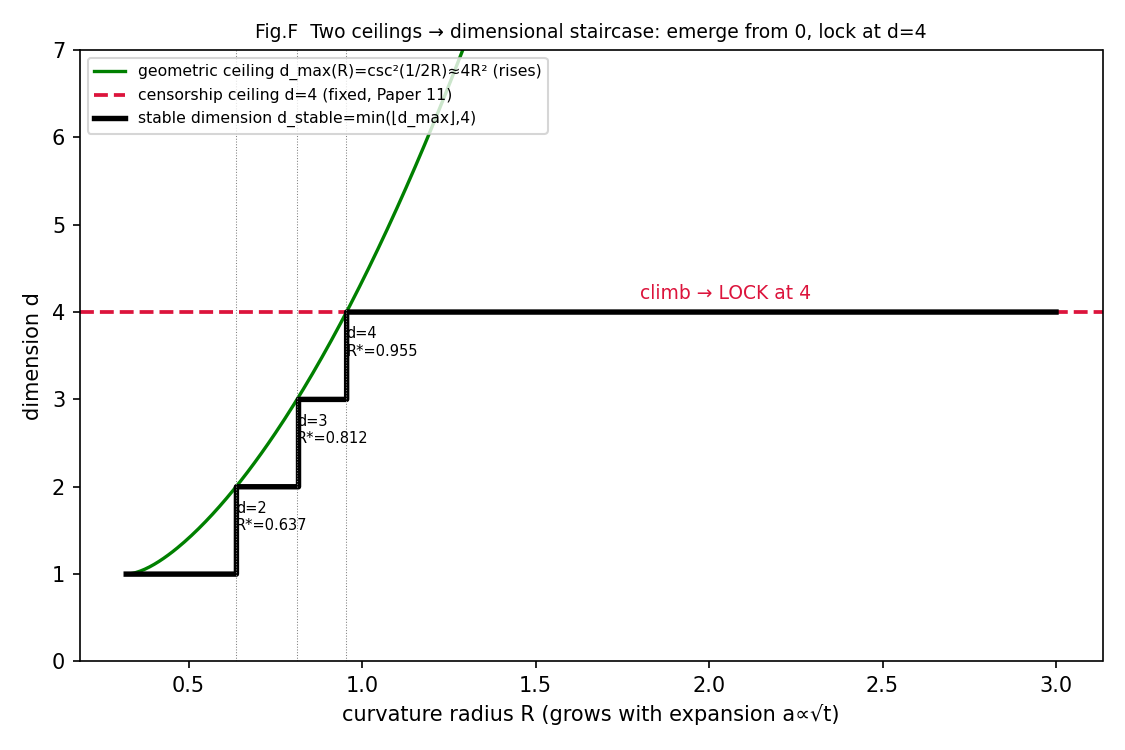
\includegraphics[width=0.88\linewidth,height=\textheight,keepaspectratio]{paper0_figF_staircase.png}

\textbf{Fig. F. The dimensional staircase (§4.7)}. The smaller of the
rising geometric ceiling d\_max(R)≈4R\(^{2}\) (green) and the fixed
censorship ceiling d=4 (red dashed, Paper 11) is the stable dimension
(thick line). With increasing R (expansion) it climbs 1→2→3→4 and locks
at 4 for R≥3/π.

\subsection{5. Connection to Papers 1--2}\label{connection-to-papers-12}

The flat count of Paper 2 assigned hypervolume 1 to each cell.
Estimating the leading term of the curvature correction in a
\textbf{mean-field approximation} (the approximation that assigns a
uniform factor V\(_{4}\)(R) to all cells),

ΔN(R) ≈ N\(_{0}\)(R)·(V\(_{4}\)(R) − 1) = N\(_{0}\)(R)/R\(^{2}\) +
O(1/R\(^{4}\)) (mean field). (11)

The smaller R, the larger the 1/R\(^{2}\) effect; it vanishes as R→∞. At
R=3, V\(_{4}\)=1.1220 (about 12\% excess).

\begin{quote}
\textbf{Explicit statement that this is a mean-field approximation
(answer to the reviewer's check on design intent)}: (11) treats each
cell as a ``pole-centered geodesic unit hypercube'' and applies a
uniform factor V\(_{4}\)(R). By the homogeneity of the sphere,
\textbf{the volume of a pole-centered geodesic cell is V\(_{4}\)(R)
regardless of position}, but the actual lattice cells of Papers 1--2 sit
on the constraint surface Σν\(^{2}\)=R\(^{2}\) at various orientations
and positions (geodesic distance χ from the pole), and the
orientation-dependent excess rate can differ cell by cell. Hence (11) is
a \textbf{leading-order, mean-field estimate}, and \textbf{an exact
version resolving shell-position and orientation dependence is future
work}. Refining the correspondence between the dimension of the
constraint surface (in 4D frequency space Σ\_\{i=1\}\^{}4
ν\(^{2}\)=R\(^{2}\) is S\(^{3}\)) and the S\^{}d(R) of this paper is
future work of the same kind. What this paper has fixed is ``the
curvature excess of a unit geodesic cell is exactly 1+c\_d/R\(^{2}\)'';
the uniform factor used to carry it into the count is an approximation.
\textbf{Note that (11) is an estimate for ``the case where the cell is
reinterpreted as a multi-dimensional geodesic cell''; the per-axis
1-dimensional logic wave + flat lattice count that the series actually
handles (§4.8) needs no correction because d=1 (c\(_{1}\)=0).} Thus §5
is future work for a hypothetical interpretation, and does not imply
that the current content of Papers 1--2 is curvature-deficient.
\end{quote}

\subsection{6. The spread ±½ in R}\label{the-spread-uxbd-in-r}

Each quantity is evaluated over {[}R−½, R+½{]}. Example for d=4
(V\(_{4}\)): at R=2, 1.6835/1.3120/1.1834; at R=5, 1.0514/1.0413/1.0340;
at R=10, 1.0112/1.0101/1.0091. Wide at small R (nonlinear), symmetric
and tiny at large R.

\subsection{7. Scope of claims}\label{scope-of-claims}

We claim: (1) distortion does not arise at d=1 and arises at d≥2 with
1/R\(^{2}\) as the leading coefficient; (2) the geodesic edge length is
invariant (1) for all dimensions, all R; (3) \textbf{the vertex angle
and the 2-face area are dimension-independent} (intrinsic 2-dimensional
quantities, cos θ=−tan\(^{2}\)(1/2R), A=V\(_{2}\)); (4) \textbf{the
volume alone is dimension-dependent}, with closed-form coefficient
c\_d=d(d−1)/12 (= the sum of the area excesses of C(d,2) 2-planes); (5)
dimension d acts not on value but also on the domain of existence
(\(R^{*}_{d}\)); (6) the excess (11) is the leading term of the
curvature correction of the flat count for the reinterpretation into
multi-dimensional geodesic cells (mean field, §5); (7) \textbf{the
per-axis 1-dimensional logic wave (Papers 5/9) is curvature-exact
because d=1 (zero distortion, any R)} --- the geometric ground (§4.8)
for Paper 9 §2.3 ``curvature consistency.'' The series avoids the seat
of distortion d≥2 by construction; (7′) \textbf{the sign and magnitude
of curvature can be inverted from the angle dimension-universally}
(curvature meter, §4.5):
θ\textgreater90°\(\Longrightarrow\)K\textgreater0,
θ\textless90°\(\Longrightarrow\)K\textless0. The direction (marking) is
unknowable but the value K is knowable from a local angle; (8)
\textbf{dimension has a ceiling
d\_max(R)=\(\lfloor\)csc\(^{2}\)(1/2R)\(\rfloor\)≈4R\(^{2}\) and an
ambiguity}, and the relative ambiguity under ±½ grows at small R (§4.6).
The candidate conjugate quantity of dimension is the per-axis curvature
load κ=sin\(^{2}\)(1/2R)≈K/4 (d·κ≤1, an observation); (9) \textbf{the
composition of the two ceilings (geometric d\_max(R)↑ and censorship
fixed 4)} yields a staircase in which dimension emerges from zero and
locks at d=4 (§4.7, an observation).

We do not claim: any physical identification / measure, probability,
amplitude (none exist in this paper).

\subsection{Appendix A: Derivation of the Jacobian (volume formula
(3))}\label{appendix-a-derivation-of-the-jacobian-volume-formula-3}

Let \(f(y)=R(y,w)/\sqrt{|y|^2+w^2}\) and \(r=\sqrt{|y|^2+w^2}\). Then
\(\partial f/\partial y_j=(R/r)\,[\,e_j^{(d+1)} - (y,w)\,y_j/r^2\,]\).
The Gram matrix \(G=J^{T}J\) is
\(G_{ij}=(R/r)^2[\,\delta_{ij} - y_i y_j/r^2\,]\), with
\(\det G=R^{2d}w^2/r^{2d+2}\). Hence
\(\sqrt{\det G}=R^{d}w/(|y|^2+w^2)^{(d+1)/2}\) is the integrand of (3).
The area of the 2-face is of the same type,
\(\sqrt{\det}=R^2 m/(y_1^2+y_2^2+m^2)^{3/2}\) (with \(m^2=R^2-2t^2\),
\(d\)-independent), giving §2 (5). \(\blacksquare\)

\subsection{Appendix B: Verification items (all
pass)}\label{appendix-b-verification-items-all-pass}

\begin{enumerate}
\def\labelenumi{\arabic{enumi}.}
\tightlist
\item
  d=2: Gauss--Bonnet area = volume integral (difference ≤
  4×10\(^{-14}\)).
\item
  Volume coefficient: c\_d=d(d−1)/12 (machine-precision agreement for
  d=2--6).
\item
  Angle dimension-independence: cos θ=−tan\(^{2}\)(1/2R), tangent-vector
  numerics agree exactly for d=2--5.
\item
  Area dimension-independence: 2-face area=V\(_{2}\) (agreement for
  d=2--5).
\item
  Limit: agreement with the flat value to 10\(^{-8}\) at R=10\(^{4}\).
  Existence threshold \(R^{*}_{d}\)=1/(2 arcsin(1/√d)).
\item
  ±½ spread: evaluated and listed for all quantities.
\item
  Angle→curvature inversion (curvature meter): negative curvature cos
  θ=+tanh\(^{2}\)(1/2R) confirmed in the hyperboloid model; the
  round-trip check agrees to machine precision for both positive and
  negative curvature. Hyperbolic has no existence threshold
  (w\(^{2}\)=R\(^{2}\)+d t\(^{2}\)\textgreater0 always,
  machine-confirmed).
\end{enumerate}

\textbf{Acknowledgments / procedure}: v0.1 was drafted as a formulation
skeleton by claude.ai. The fixing of the analytic formulas, the four
tables, the closed form of the coefficient c\_d, the
dimension-independence of angle/area, and the existence threshold are
due to independent computation by Claude Code (two-party verification
protocol). The script \texttt{paper0\_geodesic\_cell\_distortion.py} is
bundled. No physical identification is made.

\subsection{References (external)}\label{references-external}

In-series works are cited directly in the text (as the
Spherical-projection note, Papers 1/5/9/11, etc.). The external works
referenced as adjacent prior work (mathematical and conceptual
background, not a physical basis for the claims) are:

\begin{itemize}
\tightlist
\item
  {[}Carlip 2017{]} S. Carlip, \emph{Dimension and dimensional reduction
  in quantum gravity}, Classical and Quantum Gravity \textbf{34}, 193001
  (2017).
\item
  {[}Ambjørn--Jurkiewicz--Loll 2005{]} J. Ambjørn, J. Jurkiewicz, R.
  Loll, \emph{Spectral dimension of the universe}, Physical Review
  Letters \textbf{95}, 171301 (2005).
\item
  {[}Böröczky 1978{]} K. Böröczky, \emph{Packing of spheres in spaces of
  constant curvature}, Acta Mathematica Academiae Scientiarum Hungaricae
  \textbf{32}, 243--261 (1978).
\item
  {[}Coxeter 1973{]} H. S. M. Coxeter, \emph{Regular Polytopes}, 3rd
  ed., Dover (1973).
\item
  {[}Ehrenfest 1917{]} P. Ehrenfest, \emph{In what way does it become
  manifest in the fundamental laws of physics that space has three
  dimensions?}, Proceedings of the Amsterdam Academy \textbf{20},
  200--209 (1917).
\item
  {[}Tegmark 1997{]} M. Tegmark, \emph{On the dimensionality of
  spacetime}, Classical and Quantum Gravity \textbf{14}, L69--L75
  (1997).
\end{itemize}

\end{document}
